\chapter{Axes et centres de symétrie}

\section{Transformations du plan d'éléments géométriques}

%\TODO: refaire les dessins en meilleure qualité :D
Construis \dots
\begin{tasks}
    \task L'image du cercle de centre $O$ par la translation de vecteur $\overrightarrow{AB}$.
    \begin{center}
        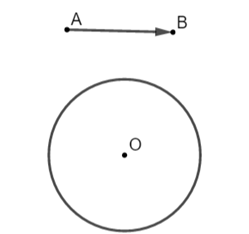
\includegraphics{axes-et-centres/img/trans_cercle.png}
    \end{center}
    \task L'image de la droite $f$ par la symétrie centrale de centre $C$.
    \begin{center}
        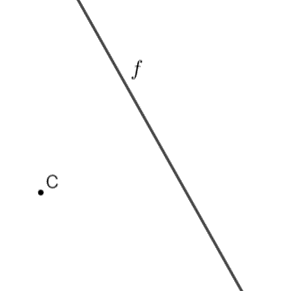
\includegraphics{axes-et-centres/img/sym_droite.png}
    \end{center}
    \task L'image de l'angle $\alpha$ par la rotation $r_{O;-30\degres}$
    \begin{center}
        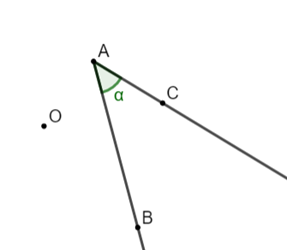
\includegraphics{axes-et-centres/img/rot_angle.png}
    \end{center}
    \task L'image du segment $[CD]$ par la symétrie orthogonale d'axe $AB$
    \begin{center}
        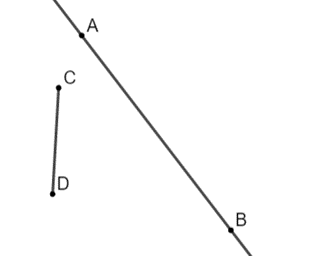
\includegraphics{axes-et-centres/img/sym_ort_segment.png}
    \end{center}
    \task L'image des droites perpendiculaires $a$ et $b$ par la rotation de centre $O$ et de $-60\degres$
    \begin{center}
        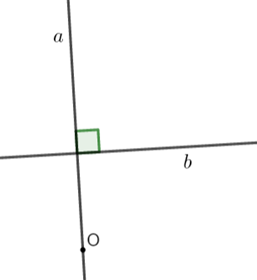
\includegraphics{axes-et-centres/img/rot_perp.png}
    \end{center}
    \task L'image des droites parallèles $e$ et $f$ par la translation de vecteur $\overrightarrow{BA}$
    \begin{center}
        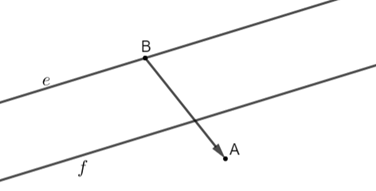
\includegraphics{axes-et-centres/img/trans_paralleles.png}
    \end{center}
\end{tasks}

\begin{exercise}
    Décode les expressions suivantes.
    \begin{tasks}
        \task $S_d(TER)=T'E'R'$
        \adf{2}
        \task $t_{\overrightarrow{BD}} ([AM])=[A'M']$
        \adf{2}
        \task $r_{A; 30\degres} (ABCD)=A'B'C'D'$
        \adf{2}
        \task $t_{\overrightarrow{AD}} (ABCD)=A'B'C'D'$
        \adf{2}
        \task $S_{CD} ([AB])=[A'B']$
        \adf{2}
        \task $r_{O; -160\degres} (fig. 1)= fig. 1'$
        \adf{2}
    \end{tasks}
\end{exercise}

\emph{Pour le résumé théorique, rendez-vous page 116.}

\section{Isométries dans les triangles}

Détermine l'ensemble des isométries admises dans les triangles suivants. Trace les éléments caractéristiques à ces isométries.

\begin{tcolorbox}
    Note : Un triangle admet une isométrie si cette isométrie envoie le triangle sur lui-même.
\end{tcolorbox}

\begin{tasks}
    \task Triangles scalènes
    \begin{center}
        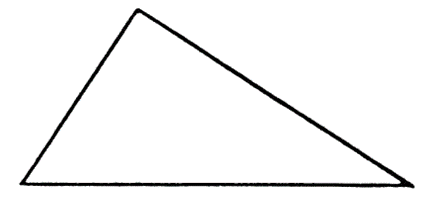
\includegraphics{axes-et-centres/img/tri_sca.png}
    \end{center} 
    \task Triangles isocèles
    \begin{center}
        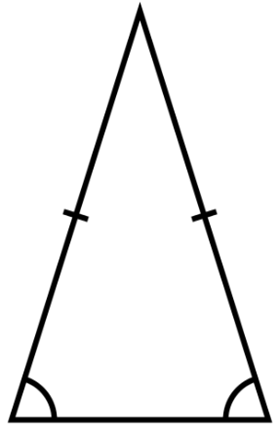
\includegraphics{axes-et-centres/img/tri_iso.png}
    \end{center} 
    \task Triangles équilatéraux
    \begin{center}
        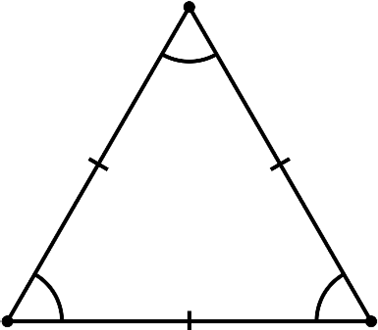
\includegraphics{axes-et-centres/img/tri_equi.png}
    \end{center}
\end{tasks}

\newpage
\section{Isométrie dans les quadrilatères}

Dresse l'arbre des quadrilatères en fonction de leurs isométries.

\emph{Pour le résumé théorique, rendez-vous pages 114 - 115.}

\newpage
\section{Les isométries dans les polygones réguliers}

\adf[Rappel : un polygone est régulier si ]{2} 

Un polygone régulier admet autant d'axes de symétrie qu'il possède de \dotfill

\exemples 
\begin{itemize}[label=$\bullet$]
    \item  Un octogone régulier admet \dots axe(s) de symétrie.
    \item  Un pentagone régulier admet \dots axe(s) de symétrie.
\end{itemize}

\adf[Un polygone régulier admet un centre de symétrie si ]{1}

\exemples
\begin{itemize}[label=$\bullet$]
    \item Un hexagone régulier admet \dots axe(s) de symétrie, alors il \dots \dots \dots \dots \dots un centre de symétrie 
    \item Un heptagone régulier admet \dots axe(s) de symétrie, alors il \dots \dots \dots \dots \dots un centre de symétrie 
\end{itemize}

\emph{Pour le résumé théorique, rendez-vous page 115.}

\section{Exercices mélangés}

\begin{exercise}
    Soit les polygones réguliers suivants. Pour chacun, indique \dots
    \begin{enumerate}
        \item leur nom
        \item le nombre d'axes de symétrie (+ trace-les)
        \item s'il admet un centre de symétrie (+ si oui, trace-le)
    \end{enumerate}
\begin{itemize}[label=, cols=2]
    \item Polygone 1 \\
    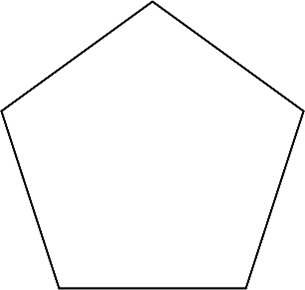
\includegraphics[height=2cm]{axes-et-centres/img/penta.png}
    \item Polygone 2 \\
    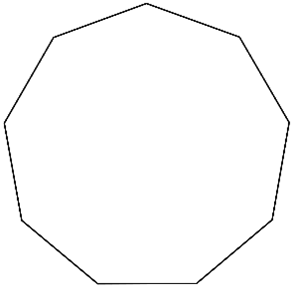
\includegraphics[height=2cm]{axes-et-centres/img/enea.png}
\end{itemize}
\end{exercise}

\begin{exercise}
    Vrai ou faux? Justifie dans tous les cas.
    \begin{enumerate}
        \item La symétrie centrale conserve les amplitudes des angles.
        \item Il n'existe aucun triangle qui possède trois axes de symétrie.
        \item Un triangle rectangle ne possède jamais d'axe de symétrie.
        \item Un quadrilatère dont les diagonales sont perpendiculaires est un losange.
        \item Un trapèze ne possède jamais d'axe de symétrie.
        \item Si mes médianes sont mes seuls axes de symétrie, je suis un losange.
        \item Un pentagone admet 5 axes de symétrie.
        \item Tout carré est un losange.
        \item Certains triangles admettent une rotation.
        \item Tout triangle isocèle possède deux axes de symétrie.
        \item Un hexagone régulier admet un centre de symétrie.
        \item Si un parallélogramme a ses diagonales de même longueur, alors ses diagonales sont des axes de symétrie.
    \end{enumerate}
\end{exercise}

\begin{exercise}
   Détermine le nombre d'axes et de centres de symétrie de ces figures. Trace-les sur cette feuille. \\
   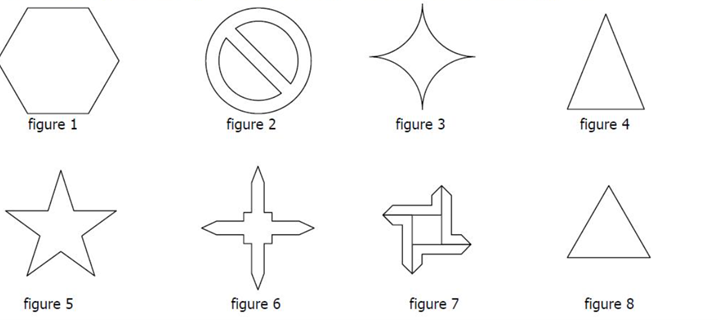
\includegraphics{axes-et-centres/img/ex_retrouver.png}
\end{exercise}

\begin{exercise}
    Combien d'axes de symétrie possède une droite? Justifie.
\end{exercise}

\begin{exercise}
    Trace une figure qui possède 8 axess de symétrie, un centre de symétrie, et qui ademt une rotation dont le centre est le même que le centre de symétrie et dont l'amplitude est de $22,5\degres$ et ses multiples.
\end{exercise}

\begin{exercise}
    Détermine le nombre exact d'axes et de centres de symétrie de ces figures. Trace-les, si possible. \\
    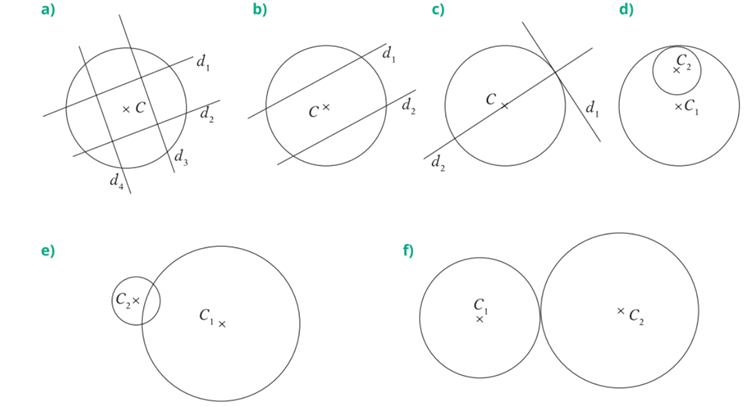
\includegraphics{axes-et-centres/img/ex_geom.png}
\end{exercise}

\begin{exercise}
    Voici une rosace que Ines a réalisé pour décorer sa farde. 

    \centering 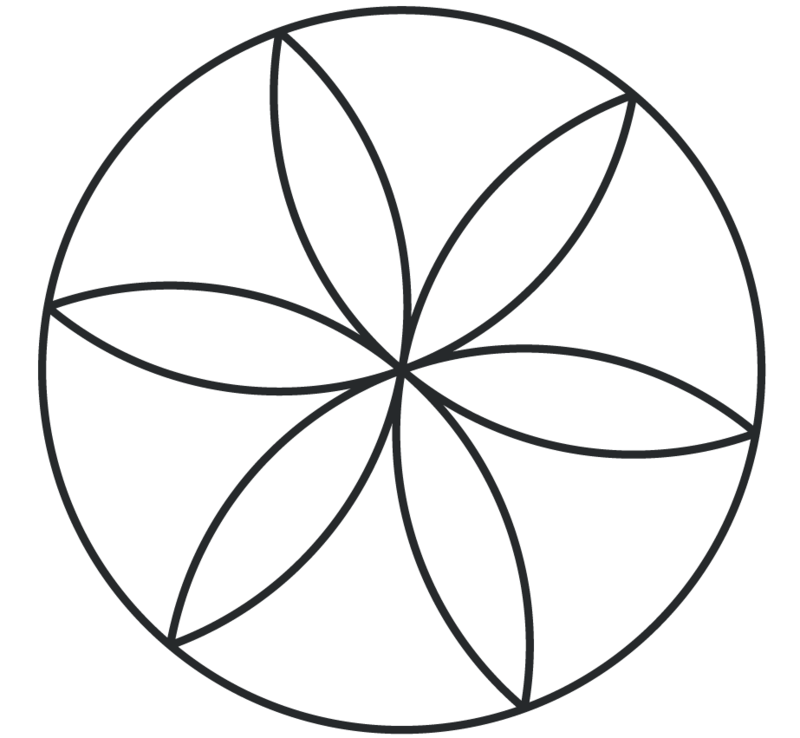
\includegraphics[height=5cm]{axes-et-centres/img/rosace.png}
    \begin{tasks}
        \task Combien d'axes de symétrie cette rosace admet-elle? Trace-les en rouge.
        \task Admet-elle une symétrie centrale? Si oui, place le centre de cette symétrie en vert.
        \task Cette rosace admet-elle d'autres isométries? Sois précis.
        \task (Dépassement) Reproduis cette rosace en prenant un rayon de 4 cm comme point de départ.
    \end{tasks}
\end{exercise}